%!TEX root=thesis.tex
\section{Minimal Surfaces}

Minimal surfaces are found at the intersection of a number of different areas in mathematics. A side-effect of this is a great number of characterizations for the definition of a minimal surface. We will first define minimal surfaces using the language of surface theory that we developed in the previous chapter, then we will continue in that same vein to view various properties of minimal surfaces using the tensors and concepts developed previously. Having done that we will take a slightly different approach to build up minimal surfaces, as surfaces of least area, which will shape and prepare us for the discussion of the next chapter.

\subsection{Minimal Surfaces in the Language of Surface Theory}

  Minimal surfaces are surfaces with mean curvature everywhere equal to zero. Without an intuitive idea about mean curvature and the implications this seems a dry, technical statement, but the reality couldn't be further from the truth. Recall the calculation of mean curvature from the previous chapter, Equation~\ref{eq:mean_curvature}. We have something of a geometric intuition built up around this definition, but the difficulty in its calculation lies with the incorporation of the Weingarten Map. With this as the medium we must travel through each time, calculation becomes cumbersome. We will show in the rest of this chapter a somewhat easier method of approaching surfaces that will lend itself well to calculation.  

\subsection{Properties of Minimal Surfaces}
  There are several properties of minimal surfaces that we'd like to highlight here.

  \begin{thm}[Theorem 3.5.7 of~\cite{Opr07}]
    If a surface of revolution $M$ is minimal, then $M$ is contained in either a plane or catenoid.
  \end{thm}

  We make the next definition to highlight an interesting fact about minimal surfaces.
  \begin{defn}
    We call a surface \emph{ruled} if, given two curves $\alpha$ and $\beta$, we can find a parameterization for the surface of the form
    \[
      \bx(s, t) = \alpha(s) + t\beta(s).
    \]
    In terms of the construction of the surface we can think of this as if we travel along $\alpha$ and at each point the surface is the sheet formed between $\alpha$ and $\beta$ mediated by the second parameter $t$. 
  \end{defn}

  \begin{thm}[Theorem 4.2.6 of~\cite{Opr07}]
    Any ruled minimal surface in $\RR^3$ is part of a plane or a helicoid.
  \end{thm}

  This next one is less of a property and more of an example, in part to motivate the discussion of the next chapter.

  \begin{ex}
    \label{ex:ennepers_surface}
    Let $M$ be the surface parameterized by the patch $\bx(u, v) = \left(u - \frac{u^3}{3} + uv^2, v - \frac{v^3}{3} + vu^2, u^2 - v^2\right)$. This is known as \emph{Enneper's Surface}. The source of our parameterization seems opaque, but we will see in the next chapter just how simple an origin this surface has. We can see one view of it in Figure~\ref{fig:ennepers_surface}.

    \begin{figure}[t] % fig: Enneper's Surface
      \centering
      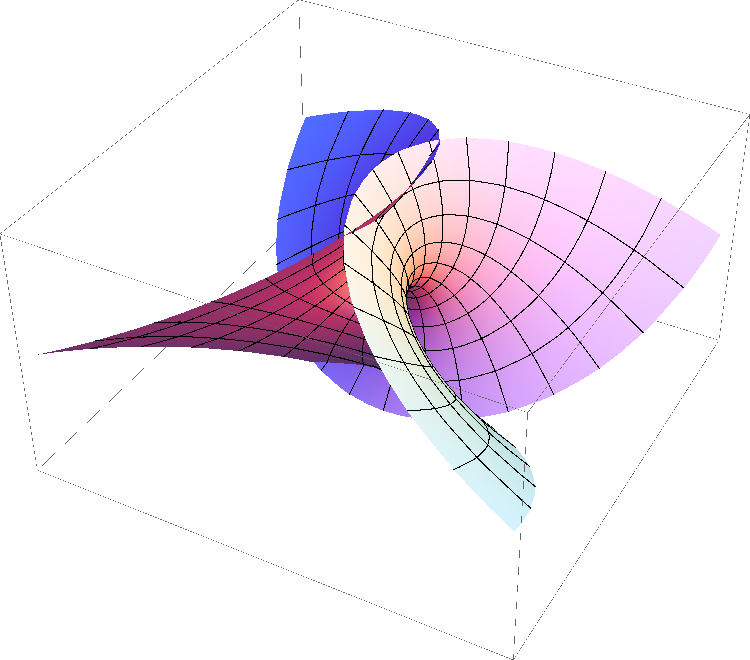
\includegraphics[width=0.5\textwidth]{figures/ennepers_surface.pdf}
      \caption{Enneper's Surface.}
      \label{fig:ennepers_surface}
    \end{figure}
  \end{ex}

\subsection{A Different Approach to Minimal Surfaces}
  \label{ss:opreaSrf}
  % TODO: Citation
  % l, m, n from Oprea07 (p88)
  % E, F, G, l, m, n, shape operator, H, K, etc.
  In the language of the previous section our examination of minimal surfaces would be something of a slog. The properties and intuition that we will build up will cover a wide range of approaches from the strictly geometric (in which case, for ease of understanding we will use the more intuitive notation of the former) to analytic. In the case of the latter we will use notation due, in part to Oprea which we will define here for convenience. Letting $u$ and $v$ refer to the first and second parameters of a simple surface, we have
  \begin{align*}
    E &= g_{11}\\
    F &= g_{12} = g_{21}\\
    G &= g_{22}\\
    l &= \bx_{uu}\cdot \bn = L_{11}\\
    m &= \bx_{uv}\cdot \bn = L_{12} = L_{21}\\
    n &= \bx_{vv}\cdot \bn = L_{22}.
  \end{align*}

  Then in terms of these new objects we have the Gaussian and Mean curvature given by
  \begin{equation*}
    K = \frac{ln - m^2}{EG - F^2}
  \end{equation*}
  and
  \begin{equation}
    \label{eq:mean_curvature2}
    H = \frac{Gl + En - 2Fm}{2(EG - F^2)},
  \end{equation}
  respectively. These may obscure some of the geometric intuition we built up earlier with our tensors but reduces our calculations to a very clean, concise language. It is with these that we move forward to introducing the following fact about minimal surfaces.

  % Minimal surface equation
  \begin{thm}
    \label{thm:minimal_surface_eq}
    A surface $M$ parameterized as a Monge patch $\bx(u, v) = (u, v, f(u, v))$ is minimal if and only if
    \begin{equation*}
      f_{uu}\left(1 + f_v^2\right) - 2f_uf_vf_{uv} + f_{vv}\left(1 + f_u^2\right) = 0.
    \end{equation*}
  \end{thm}
  \begin{proof}
    We simply make the necessary calculations and get
    \begin{align*}
      \bx_u &= (1, 0, f_u)\\
      \bx_v &= (0, 1, f_v)\\
      \bx_{uu} &= (0, 0, f_{uu})\\
      \bx_{uv} &= (0, 0, f_{uv})\\
      \bx_{vv} &= (0, 0, f_{vv})\\
      \bx_u \times \bx_v &= (-f_u, -f_v, 1).
    \end{align*}
    Then, calculating the unit normal and the rest of the items needed for $H$ above (letting $w = \sqrt{1 + f_u^2 + f_v^2}$, we find
    \begin{align*}
      \bn &= \frac{(-f_u, -f_v, 1)}{w}\\
      E &= 1 + f_u^2\\
      F &= f_uf_v\\
      G &= 1 + f_v^2\\
      \ell &= \frac{f_{uu}}{w}\\
      m &= \frac{f_{uv}}{w}\\
      n &= \frac{f_{vv}}{w},
    \end{align*}
    and finally
    \begin{align*}
      H &= \frac{Gl + En - 2Fm}{2(EG - F^2)}\\
      &= \frac{(1 + f_v^2)f_{uu} + (1 + f_u^2)f_{vv} - 2f_uf_vf_{uv}}{2w^3}.
    \end{align*}
    Then since a surface is minimal when $H = 0$, this implies that a surface is minimal when 
    \[
      (1 + f_v^2)f_{uu} + (1 + f_u^2)f_{vv} - 2f_uf_vf_{uv} = 0,
    \]
    as required.
  \end{proof}
